\documentclass[a4paper, journal]{IEEEtran}
\usepackage[margin=0.75in]{geometry}
\IEEEoverridecommandlockouts
% The preceding line is only needed to identify funding in the first footnote. If that is unneeded, please comment it out.
\usepackage{cite}
\usepackage{amsmath,amssymb,amsfonts}
\usepackage{algorithmic}
\usepackage{graphicx}
\usepackage{textcomp}
\usepackage{listings}
\usepackage{xcolor}
\usepackage{booktabs}
\usepackage{tikz}
\usepackage{times}
\usepackage{newtxmath}


\definecolor{codegreen}{rgb}{0,0.6,0}
\definecolor{codegray}{rgb}{0.5,0.5,0.5}
\definecolor{codepurple}{rgb}{0.58,0,0.82}
\definecolor{backcolour}{rgb}{0.95,0.95,0.92}

\lstset{
  language=Python,
  breaklines=true,
  breakatwhitespace=true,
  basicstyle=\ttfamily\footnotesize,
  keywordstyle=\color{codepurple},
  commentstyle=\color{codegreen},
  stringstyle=\color{red},
  captionpos=b,
  frame=single,
  showstringspaces=false,
  tabsize=4
}


\hyphenation{op-tical net-works semi-conduc-tor IEEE-Xplore}
\def\BibTeX{{\rm B\kern-.05em{\sc i\kern-.025em b}\kern-.08em
    T\kern-.1667em\lower.7ex\hbox{E}\kern-.125emX}}
\usepackage{balance}
\begin{document}

\title{Multilayer Perceptron}
\author{
\IEEEauthorblockN{Dinanath Padhya\IEEEauthorrefmark{1}, Krishna Acharya\IEEEauthorrefmark{2}} \\
\IEEEauthorblockA{\IEEEauthorrefmark{1}THA078BEI010 \quad \IEEEauthorrefmark{2}THA078BEI020\\
Department of Electronics, Communication and Information Engineering\\
Thapathali Campus, IOE, Tribhuvan University, Nepal\\
}}

\maketitle

\begin{abstract}

\end{abstract}
\begin{IEEEkeywords}
\end{IEEEkeywords}

\section{Introduction}

\subsection{Background}

\subsection{Literature Review}

\subsection{Objectives}
This laboratory experiment aims to:
\begin{itemize}
    \item Objective 1

\end{itemize}


\section{Methodology}

\subsection{Implementation Environment}


\section{Theoretical Background}

\subsection{Activation Functions}
Activation functions are mathematical functions applied to the output of each neuron in a neural network layer. Their primary purpose is to introduce non-linearity into the model, enabling neural networks to approximate complex, non-linear mappings between inputs and outputs. Without activation functions, a neural network, regardless of its depth, would behave as a single linear transformation, severely limiting its representational power. \\

\subsubsection{Sigmoid}
The sigmoid function is a smooth, S-shaped curve that maps any real-valued input to the range $(0, c)$, making it especially suitable for binary classification tasks. The general form of the sigmoid function with parameters $a$, $b$, and $c$ is:
\begin{equation}
\sigma(x) = \frac{c}{a + be^{-x}}
\end{equation}
where $a$, $b$, and $c$ are constants that control the curve's shape:

\begin{itemize}
    \item \textbf{Parameter $c$} sets the upper asymptote (maximum value) of the function.
    \item \textbf{Parameter $a$} affects the lower asymptote; when $a=1$, the function ranges from $0$ to $c$.
    \item \textbf{Parameter $b$} controls the steepness and direction; increasing $b$ makes the curve steeper, while negative $b$ reflects it horizontally.
\end{itemize}

The standard sigmoid, with $a=1$, $b=1$, $c=1$, produces the classic S-curve from $0$ to $1$, crossing $0.5$ at $x=0$ (see Figure~\ref{fig:sigmoid}).

\begin{figure}[h]
\centering
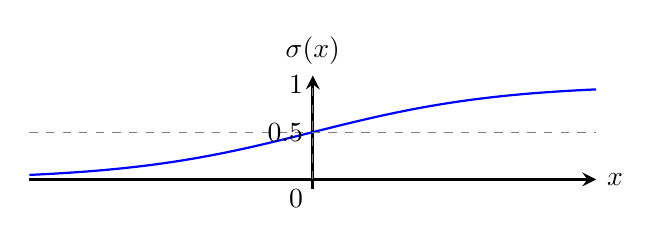
\begin{tikzpicture}[scale=1.2, axis/.style={very thick, ->, >=stealth}]
% Axes
\draw[axis] (-3,0) -- (3,0) node[right] {$x$};
\draw[axis] (0,-0.1) -- (0,1.1) node[above] {$\sigma(x)$};
% Sigmoid curve
\draw[thick, blue, domain=-3:3, samples=100, smooth] plot (\x,{1/(1+exp(-\x))});
% Dashed lines for y=0.5
\draw[dashed, gray] (-3,0.5) -- (3,0.5);
\draw[dashed, gray] (0,0) -- (0,1);
% Labels
\node[left] at (0,1) {$1$};
\node[left] at (0,0.5) {$0.5$};
\node[below left] at (0,0) {$0$};
\end{tikzpicture}
\caption{Sigmoid Activation Function}
\label{fig:sigmoid}
\end{figure}

\begin{figure}[h]
\centering
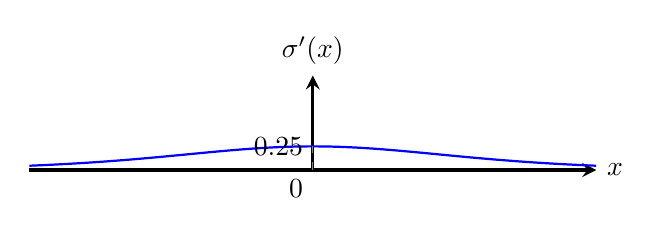
\begin{tikzpicture}[scale=1.2, axis/.style={very thick, ->, >=stealth}]
% Axes
\draw[axis] (-3,0) -- (3,0) node[right] {$x$};
\draw[axis] (0,0) -- (0,1) node[above] {$\sigma'(x)$};
% Derivative of sigmoid curve
\draw[thick, blue, domain=-3:3, samples=100, smooth] plot (\x,{exp(-\x)/(1+exp(-\x))^2});
% Additional information
\draw[dashed, gray] (0,0) -- (0,0.25);
\node[left] at (0,0.25) {$0.25$};
\node[below left] at (0,0) {$0$};
\end{tikzpicture}
\caption{Derivative of Sigmoid Activation Function: $\sigma'(x) = \sigma(x)(1 - \sigma(x))$}
\label{fig:sigmoid_derivative}
\end{figure}
\begin{equation}
\sigma'(x) = \sigma(x)(1 - \sigma(x))
\end{equation}

The sigmoid function is widely used in neural networks due to its differentiability and well-defined gradient, which is essential for backpropagation:




\subsubsection{Tanh}
Tanh outputs values in $(-1, 1)$, centering the data and often leading to faster convergence than sigmoid:
\begin{equation}
\tanh(x) = \frac{e^{x} - e^{-x}}{e^{x} + e^{-x}}
\end{equation}

\begin{figure}[h]
\centering
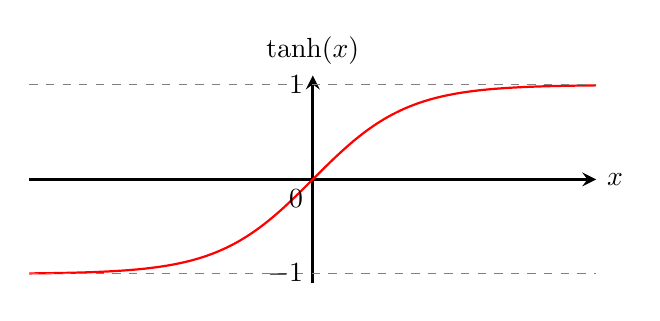
\begin{tikzpicture}[scale=1.2, axis/.style={very thick, ->, >=stealth}]
% Axes
\draw[axis] (-3,0) -- (3,0) node[right] {$x$};
\draw[axis] (0,-1.1) -- (0,1.1) node[above] {$\tanh(x)$};
% Tanh curve
\draw[thick, red, domain=-3:3, samples=100, smooth] plot (\x,{tanh(\x)});
% Horizontal asymptotes
\draw[dashed, gray] (-3,1) -- (3,1);
\draw[dashed, gray] (-3,-1) -- (3,-1);
% Labels
\node[left] at (0,1) {$1$};
\node[left] at (0,-1) {$-1$};
\node[below left] at (0,0) {$0$};
\end{tikzpicture}
\caption{Tanh Activation Function}
\label{fig:tanh}
\end{figure}


\begin{figure}[h]
\centering
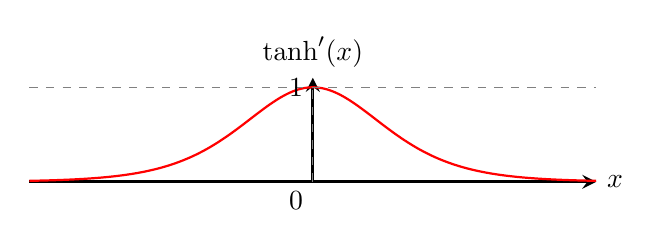
\begin{tikzpicture}[scale=1.2, axis/.style={very thick, ->, >=stealth}]
% Axes
\draw[axis] (-3,0) -- (3,0) node[right] {$x$};
\draw[axis] (0,0) -- (0,1.1) node[above] {$\tanh'(x)$};
% Derivative of tanh curve
\draw[thick, red, domain=-3:3, samples=100, smooth] plot (\x,{1-tanh(\x)*tanh(\x)});
% Maximum value
\draw[dashed, gray] (-3,1) -- (3,1);
\draw[dashed, gray] (0,0) -- (0,1);
% Labels
\node[left] at (0,1) {$1$};
\node[below left] at (0,0) {$0$};
\end{tikzpicture}
\caption{Derivative of Tanh Activation Function: $\tanh'(x) = 1 - \tanh^2(x)$}
\label{fig:tanh_derivative}
\end{figure}


Its derivative is:
\begin{equation}
\tanh'(x) = 1 - \tanh^2(x)
\end{equation}

Like sigmoid, it can also suffer from vanishing gradients.

\subsubsection{ReLU (Rectified Linear Unit)}
ReLU is widely used due to its simplicity and effectiveness:
\begin{equation}
f(x) = \max(0, x)
\end{equation}

\begin{figure}[h]
\centering
\begin{tikzpicture}[scale=1.2, axis/.style={very thick, ->, >=stealth}]
% Axes
\draw[axis] (-3,0) -- (3,0) node[right] {$x$};
\draw[axis] (0,0) -- (0,3) node[above] {$f(x)$};
% ReLU curve
\draw[thick, green!60!black, domain=-3:0, samples=2] plot (\x,{0});
\draw[thick, green!60!black, domain=0:3, samples=2] plot (\x,{\x});
% Point of non-differentiability
\filldraw[green!60!black] (0,0) circle (1.5pt);
% Labels
\node[left] at (0,0) {$0$};
\end{tikzpicture}
\caption{ReLU Activation Function: $f(x) = \max(0, x)$}
\label{fig:relu}
\end{figure}

\begin{figure}[h]
\centering
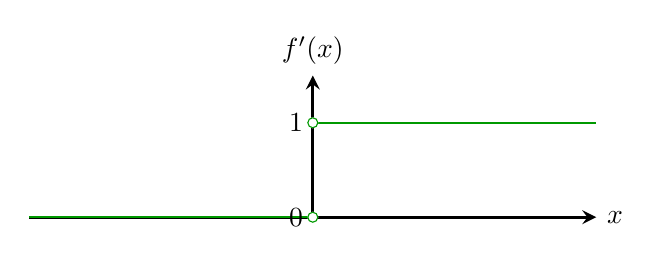
\begin{tikzpicture}[scale=1.2, axis/.style={very thick, ->, >=stealth}]
% Axes
\draw[axis] (-3,0) -- (3,0) node[right] {$x$};
\draw[axis] (0,0) -- (0,1.5) node[above] {$f'(x)$};
% ReLU derivative
\draw[thick, green!60!black, domain=-3:0, samples=2] plot (\x,{0});
\draw[thick, green!60!black, domain=0:3, samples=2] plot (\x,{1});
% Point of discontinuity
\filldraw[white] (0,0) circle (1.5pt);
\draw[green!60!black] (0,0) circle (1.5pt);
\filldraw[white] (0,1) circle (1.5pt);
\draw[green!60!black] (0,1) circle (1.5pt);
% Labels
\node[left] at (0,1) {$1$};
\node[left] at (0,0) {$0$};
\end{tikzpicture}
\caption{Derivative of ReLU Activation Function}
\label{fig:relu_derivative}
\end{figure}

It outputs zero for negative inputs and the input itself for positive values. Its derivative is:
\begin{equation}
f'(x) = 
\begin{cases} 
1 & \text{if } x > 0 \\
0 & \text{otherwise}
\end{cases}
\end{equation}

ReLU helps mitigate the vanishing gradient problem but can lead to dead neurons if too many outputs become zero.

\subsubsection{Leaky ReLU}
This variant allows a small, non-zero gradient when the unit is not active:
\begin{equation}
f(x) = \max(\alpha x, x)
\end{equation}

\begin{figure}[h]
\centering
\begin{tikzpicture}[scale=1.2, axis/.style={very thick, ->, >=stealth}]
% Axes
\draw[axis] (-3,0) -- (3,0) node[right] {$x$};
\draw[axis] (0,-1) -- (0,3) node[above] {$f(x)$};
% Leaky ReLU curve
\draw[thick, purple, domain=-3:0, samples=2] plot (\x,{0.01*\x});
\draw[thick, purple, domain=0:3, samples=2] plot (\x,{\x});
% Point of non-differentiability
\filldraw[purple] (0,0) circle (1.5pt);
% Labels
\node[left] at (0,0) {$0$};
\end{tikzpicture}
\caption{Leaky ReLU Activation Function: $f(x) = \max(\alpha x, x)$ with $\alpha = 0.01$}
\label{fig:leaky_relu}
\end{figure}

\begin{figure}[h]
\centering
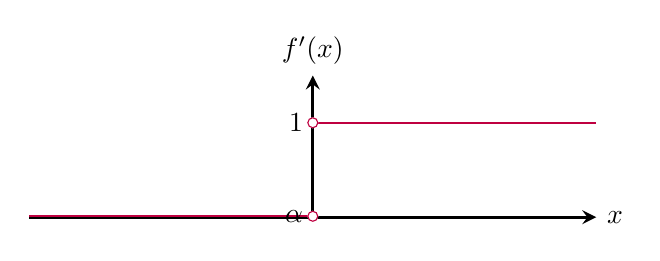
\begin{tikzpicture}[scale=1.2, axis/.style={very thick, ->, >=stealth}]
% Axes
\draw[axis] (-3,0) -- (3,0) node[right] {$x$};
\draw[axis] (0,0) -- (0,1.5) node[above] {$f'(x)$};
% Leaky ReLU derivative
\draw[thick, purple, domain=-3:0, samples=2] plot (\x,{0.01});
\draw[thick, purple, domain=0:3, samples=2] plot (\x,{1});
% Point of discontinuity
\filldraw[white] (0,0.01) circle (1.5pt);
\draw[purple] (0,0.01) circle (1.5pt);
\filldraw[white] (0,1) circle (1.5pt);
\draw[purple] (0,1) circle (1.5pt);
% Labels
\node[left] at (0,1) {$1$};
\node[left] at (0,0.01) {$\alpha$};
\end{tikzpicture}
\caption{Derivative of Leaky ReLU Activation Function: $f'(x) = \begin{cases} 1 & \text{if } x > 0 \\ \alpha & \text{otherwise} \end{cases}$}
\label{fig:leaky_relu_derivative}
\end{figure}

Where $\alpha$ is a small constant (e.g., 0.01). This helps address the dead neuron issue.

\subsubsection{Softmax}
Used in the output layer for multi-class classification:
\begin{equation}
\mathrm{softmax}(x_i) = \frac{e^{x_i}}{\sum_j e^{x_j}}
\end{equation}

Softmax converts logits into probabilities that sum to 1. Its derivative is more complex, involving the Jacobian matrix.

Activation functions are chosen based on the problem type and network architecture. Their derivatives are essential for gradient-based optimization, as they determine how errors are propagated backward through the network during training.

\subsection{Pseudo-Random Number Generators (PRNGs)}
Pseudo-random number generators (PRNGs) are deterministic algorithms that produce sequences of numbers with properties approximating true randomness. While not truly random (as they're based on mathematical formulas), high-quality PRNGs produce sequences that pass statistical tests for randomness. In neural network development and machine learning broadly, PRNGs serve several critical functions:

\begin{itemize}
    \item \textbf{Weight Initialization:} Neural networks require random initial weights to break symmetry between neurons. If all weights started with identical values, neurons in the same layer would compute identical outputs and gradients, making the network ineffective. Common initialization strategies like He, Xavier/Glorot, and standard normal distributions all rely on PRNGs.
    
    \item \textbf{Dataset Shuffling:} Random shuffling of training data prevents the network from learning artificial patterns based on the order of samples. This is particularly important in mini-batch gradient descent, where the composition of each batch significantly affects convergence.
    
    \item \textbf{Data Augmentation:} Random transformations (rotations, translations, noise addition) create variations of training examples, effectively expanding the dataset and improving model robustness.
    
    \item \textbf{Dropout Regularization:} This technique randomly deactivates neurons during training with probability $p$, requiring high-quality random number generation to be effective.
    
    \item \textbf{Stochastic Processes:} Many advanced ML techniques like stochastic gradient descent, Monte Carlo methods, and genetic algorithms rely on randomness for exploration of the parameter space.
    \item Initializing model weights randomly to break symmetry and ensure diverse learning.
    \item Shuffling datasets to prevent learning order bias.
\item Generating synthetic data for experiments and augmentation.
\end{itemize}
% ...existing code...
% ...existing code...
\texttt{torch.rand} is a PyTorch function that returns a tensor filled with random numbers from a uniform distribution over \([0,1)\). Since PRNGs are deterministic given a seed, setting the random seed \texttt{torch.manual\_seed(42)} ensures reproducibility of experiments, which is vital for scientific research and debugging.`'
% ...existing code...
% ...existing code...



\subsection{Encoding}
Machine learning models require numerical input. For categorical data, encoding methods are used:
\begin{itemize}
    \item \textbf{Label Encoding (LE):} Each unique category is assigned an integer value. For example, [cat, dog, fish] $\rightarrow$ [0, 1, 2]. This method is simple but can introduce unintended ordinal relationships between categories, which may mislead some models.
    \item \textbf{One-Hot Encoding (OHE):} Each category is represented as a binary vector with a single 1 and the rest 0s. For example, [cat, dog, fish] $\rightarrow$ [1,0,0], [0,1,0], [0,0,1]. OHE avoids ordinal relationships and is preferred for nominal categorical variables, especially in neural networks.
\end{itemize}

In classification tasks, especially with neural networks, one-hot encoding is often used for target labels. For example, in a three-class problem, the label 2 would be encoded as [0, 0, 1]. This format is compatible with loss functions like cross-entropy, which expect probability distributions as targets.

\subsection{Loss Functions}
Loss functions, also known as cost or objective functions, measure the discrepancy between the model's predictions and the actual target values. They guide the optimization process by providing a signal (the loss) that the optimizer seeks to minimize.

\subsubsection{Mean Squared Error (MSE)}
\begin{equation}
L = \frac{1}{n}\sum_{i=1}^n (y_i - \hat{y}_i)^2
\end{equation}
Used for regression, MSE penalizes larger errors more heavily. Its derivative with respect to \(\hat{y}\) is:
\begin{equation}
\frac{\partial L}{\partial \hat{y}} = -2(y - \hat{y})
\end{equation}

\subsubsection{Cross-Entropy Loss}
\begin{equation}
L = -\sum_{i} y_i \log(\hat{y}_i)
\end{equation}
Used for classification, especially with one-hot encoded targets. It measures the dissimilarity between the true distribution \(y\) and the predicted distribution \(\hat{y}\). For binary classification, it reduces to the binary cross-entropy (log loss).
Derivative of Cross-Entropy Loss
\
Assuming the logits \(\mathbf{z}\) produce \(\boldsymbol{\hat{y}}\) via softmax, the derivative with respect to \(z_i\) is:
\[
\frac{\partial L}{\partial z_i} = \hat{y}_i - y_i.
\]

\subsubsection{Negative Log Likelihood (NLL)}
Often used with softmax for multi-class classification. It quantifies the likelihood of the observed data under the parameterized model.

The choice of loss function depends on the task (regression, binary classification, multi-class classification) and directly affects the learning dynamics. The derivatives of loss functions are used in backpropagation to compute gradients for parameter updates.

% Figure suggestion: Plot of MSE and cross-entropy loss curves and their derivatives.

\subsubsection{Optimizers}
Optimizers are algorithms that adjust the parameters (weights and biases) of a neural network to minimize the loss function. They use the gradients computed during backpropagation to update parameters in the direction that reduces the loss.

Key optimizers include:
\begin{itemize}
    \item \textbf{Stochastic Gradient Descent (SGD):} The basic optimizer. Parameters are updated as $w \leftarrow w - \eta \nabla L$, where $\eta$ is the learning rate. SGD can be noisy but helps escape local minima. Mini-batch SGD is commonly used for efficiency.
    \item \textbf{Momentum:} Accelerates SGD by adding a fraction of the previous update to the current one, helping to smooth out oscillations.
    \item \textbf{RMSprop:} Adapts the learning rate for each parameter by dividing the gradient by a running average of its recent magnitude. This helps in dealing with non-stationary objectives and speeds up convergence.
    \item \textbf{Adagrad:} Adapts learning rates based on the frequency of parameter updates, performing larger updates for infrequent parameters.
    \item \textbf{Adadelta:} An extension of Adagrad that seeks to reduce its aggressive, monotonically decreasing learning rate.
    \item \textbf{Adam:} Combines the benefits of RMSprop and momentum. Maintains running averages of both the gradients and their squares, and uses these to compute adaptive learning rates for each parameter. Adam is widely used due to its robustness and efficiency.
\end{itemize}

Optimizers are essential because manual updates are impractical for large models and datasets. The choice of optimizer affects convergence speed, stability, and final model performance. For example, Adam often converges faster and more reliably than vanilla SGD, especially in deep networks.

% Table suggestion: Comparison of optimizer formulas and properties.

\subsubsection{Training and Evaluation Loops}
The process of training a neural network involves iteratively updating model parameters to minimize the loss. The standard pipeline consists of:
\begin{enumerate}
    \item \textbf{Data Processing:} Data is cleaned, normalized, and encoded (e.g., one-hot encoding for labels).
    \item \textbf{Model Forward Pass:} Input data is passed through the network to obtain predictions.
    \item \textbf{Loss Calculation:} The loss function computes the error between predictions and true labels.
    \item \textbf{Backpropagation:} The gradients of the loss with respect to each parameter are computed using the chain rule.
    \item \textbf{Optimizer Step:} The optimizer updates the parameters using the computed gradients.
    \item \textbf{Weight Update:} Parameters are adjusted to reduce the loss.
\end{enumerate}
This sequence is repeated for multiple epochs over the training data. After training, the model is evaluated on a separate validation or test set to assess its generalization performance. Evaluation metrics (e.g., accuracy, precision, recall) are used to quantify performance.

% Figure suggestion: Diagram of the training and evaluation pipeline.

\subsubsection{Backpropagation and Gradients}
Backpropagation is the core algorithm for training neural networks. It efficiently computes the gradients of the loss function with respect to each parameter by applying the chain rule of calculus through the network's layers.

For a simple logistic regression model:
\begin{align*}
    &\text{1. Compute the derivative of the loss with respect to the output:}\quad \frac{\partial L}{\partial \hat{y}} \\
    &\text{2. Compute the derivative of the output with respect to the input to the activation:}\quad \frac{\partial \hat{y}}{\partial z} \\
    &\text{3. Compute the derivative of the input with respect to each weight:}\quad \frac{\partial z}{\partial w_i}
\end{align*}
The total gradient for each weight is the product of these derivatives (chain rule):
\begin{align*}
    \frac{\partial L}{\partial w_i} = \frac{\partial L}{\partial \hat{y}} \cdot \frac{\partial \hat{y}}{\partial z} \cdot \frac{\partial z}{\partial w_i}
\end{align*}

This process is repeated for all parameters in the network. The gradients are then used by the optimizer to update the weights, gradually reducing the loss and improving the model's predictions. Backpropagation is efficient due to dynamic programming (caching intermediate results), making it feasible to train deep networks.

\subsection*{Dataset}


\section{Experiment \& Model Implementation}




\section{Results}


\section{Conclusion}



\bibliographystyle{IEEEtran}
\bibliography{ref}

\end{document}